\section{The research loop: \CR}
\label{sec:loop}

\subsection{Objects}
A \emph{subject} $s$ is a deceased person with name variants, birth and death years with precision, places, family notes and a research question. The \emph{evidence state} $R_t$ is the set of findings so far. A finding has a source, a mode (\emph{live}, from a public endpoint, or \emph{stub}, from a curated fixture or a source that needs a human), a status, claims (each with a tier: documented, told, lore or inferred) and citations (URL, title, item id, snippet, and a name-match strength). The \emph{question graph} $G=(V,E)$ has one node per question. A node $v$ carries its text $q_v$, its parent $p(v)$, the finding that sparked it $f_v$ (the ``because'', quoted), a plan $\pi_v=(\text{handler},\text{query})$, a status in \{pending, running, answered, no\_lead, stub, error, skipped\}, its answer, citations, snippets, attempts and failures, its depth $d(v)$ and its round. $E$ holds the edges $(p(v),v)$. The root is $s$; level 0 is the circuit checklist. The \emph{question memory} $M$ holds every question ever asked for this subject key (and, for H3, similar subjects), keyed by a canonical key $\kappa(q)$. The budgets are the breadth $b$ (questions picked per expanded node), the depth limit $d_{\max}$, the node budget $N$, the tool-call budget $B$, the wall-clock budget $T$, and the pause between levels $\tau$, a durable timer.

\subsection{Generate, dedupe, score, select}
\paragraph{Generator.} $g(s,R,v,M)$ returns candidate questions $C$. \emph{Grounding constraint:} every $c\in C$ must name a finding $f_c\in R$, or the node or checklist gap that sparked it, and quote it. A candidate with no spark is rejected and counted. This is the difference from free brainstorming: curiosity is anchored to evidence, so the graph is auditable. The rule-based generator (the one measured in the pilot) has lead templates keyed on what a finding contains: a military unit leads to regimental books and newspapers; a ship to voyages and crew lists; a ``son of A and B'' line to the parents; a marriage, school or congregation to its registers; a death year to an obituary; a book hit to a search inside that book for the page. A grounded model generator is implemented behind the same activity and must return a spark id and a quote that the code checks against the spark text; it has not been measured.

\paragraph{Dedupe.} Drop $c$ if $\kappa(c)\in M$ or $\kappa(c)$ is already in $V$. $\kappa$ is a normalised template key, for example \texttt{unit-books:12th-connecticut-infantry}. For model-written questions, which reword freely, a near-duplicate test also drops $c$ when its similarity to any asked question is at least $\theta$; we use the larger of word-set Jaccard and a character-sequence ratio, with $\theta=0.85$.

\paragraph{Score.} In general,
\begin{multline}
\mathrm{score}(c)=w_y\,\mathrm{yield}(\mathrm{tmpl}(c))+w_n\,\mathrm{novelty}(c)\\
+w_r\,\mathrm{rel}(c,\text{question})+w_t\,\mathrm{tier}(c)-w_c\,\mathrm{cost}(c),
\end{multline}
with $\mathrm{novelty}(c)=1-\max_{a\in M\cup V}\mathrm{sim}(c,a)$. The current implementation uses fixed integer template scores plus 2 when the user's research question mentions the topic; the weighted form is the general case that the ablations vary.

\paragraph{Select.} Pick the top $b$ live candidates, plus up to 2 stub candidates (questions that need a human or a letter, such as a pension file at the National Archives), and hold back up to 12 as ``not yet asked'', shown in the dashboard.

\subsection{Expand, nudge, stop}
\paragraph{Expansion is the recursion.} For each picked node, investigate it (an activity with retries), add its finding to $R$, and call $g$ again \emph{conditioned on that node's own finding}. That conditioning gives lead chains: ``book found'' leads to ``does that book name him, and on which page?'', which leads to ``are you sure it is the same Erastus?''.

\paragraph{Built-in nudges.} An answered node whose match is weak (surname only, or a newspaper hit without place) spawns an ``Are you sure?'' verification question. Every node spawns a ``Where else might this be?'' question that switches source family, books to newspapers or back. A checklist gap spawns ``Still nothing on $X$: where else could it be?''. A person can inject a question at any time with a signal (``Dig here first''); it joins the next level and is followed to the same depth.

\paragraph{Stopping rules.} Each run records which rule fired: (1) the frontier is empty, no new grounded, non-duplicate question; (2) $|V|$ reaches $N$; (3) the tool-call count reaches $B$; (4) elapsed time reaches $T$; (5) depth reaches $d_{\max}$. Proposed but not implemented: (6) marginal yield, new verified records per node, below $\epsilon$ for $k$ consecutive levels.

\begin{algorithm*}[t]
\caption{\CR as a durable workflow. Lines marked $\triangleright$ are activities: recorded in event history, retried, never repeated after they finish.}
\label{alg:cr}
\footnotesize
\begin{algorithmic}[1]
\Procedure{CuriosityRecursion}{$s$, circuits, $b$, $d_{\max}$, $N$, $B$, $T$, $\tau$, $M$}
\State \textsc{Gate}$(s)$ \Comment{living-person gate, deterministic, in workflow code}
\State $R \gets$ \textsc{RunChecklist}(circuits$(s)$) $\triangleright$ \Comment{level 0, parallel, each step retried}
\State $F \gets$ \textsc{Reask}$(M, s, \text{limit}=b)$ \Comment{memory: recheck earlier top-level questions first}
\State $F \gets F \cup \textsc{Select}(\textsc{Dedupe}(g(s,R,\text{root},M),M),b)$ $\triangleright$
\While{$F \neq \emptyset$}
  \State $\mathit{next} \gets [\,]$
  \ForAll{$v \in F$ \textbf{in parallel}}
    \State $v.\mathit{finding} \gets$ \textsc{Investigate}$(v)$ $\triangleright$ \Comment{retry with backoff}
    \State $R \gets R \cup \{v.\mathit{finding}\}$
    \If{$d(v) < d_{\max}$} $\mathit{next} \gets \mathit{next} \cup \textsc{Select}(\textsc{Dedupe}(g(s,R,v,M),M),b)$ $\triangleright$ \EndIf
  \EndFor
  \State \textsc{Persist}$(V, M)$ $\triangleright$ \Comment{every level, every question}
  \If{$\mathit{next}=\emptyset$ \textbf{or} $|V|\ge N$ \textbf{or} calls $\ge B$ \textbf{or} time $\ge T$} \textbf{break} \EndIf
  \State \textsc{DurableSleep}$(\tau)$ \Comment{survives restarts; minutes to weeks}
  \State $F \gets \mathit{next} \cup \textsc{HumanRedirects}()$
\EndWhile
\State $\mathit{report} \gets$ \textsc{Compose}$(R)$ $\triangleright$ \Comment{only documented claims become prose; leads quoted as leads}
\State wait for an \textsc{Approve} or \textsc{Reject} signal, with timeout; \textsc{Redirect} signals reopen the loop
\State \Return $\mathit{report}, G$
\EndProcedure
\end{algorithmic}
\end{algorithm*}

\subsection{Worked example}
\label{sec:worked}
\Cref{fig:graph} is a real run for Erastus W.\ Burnham (1834 to 1921) on the Civil War veteran circuit (run \texttt{studio-erastus-w-burnham-1126-110934}, 25 nodes). Level 0 ran 16 checklist steps; its unit facts came from a curated fixture and are labelled stub. Memory re-asked three top-level questions from earlier runs. One of them, \textit{r3}, asked ``Which books cover the 12th Connecticut Infantry, and do they name him?'' and found two candidate books on Internet Archive by catalogue title search (live). At level 2, \textit{r3.2} searched inside one of them, \emph{The Twelfth Regiment, Connecticut Volunteer Infantry in the War of the Rebellion}, and found a roster on page image 14 that reads, verbatim, ``Burke, John Burnham, Erastus W.\ Carlan, John''. The roster lists surname first in alphabetical order, so ``Burnham, Erastus W.''\ is an entry. Its first attempts failed with simulated 503 errors and Temporal retried them. This is a T1 find: the roster is online, but in no name index the agent was given. It is a lead, a full-name match, not an identification.

\begin{figure*}[t]
\centering
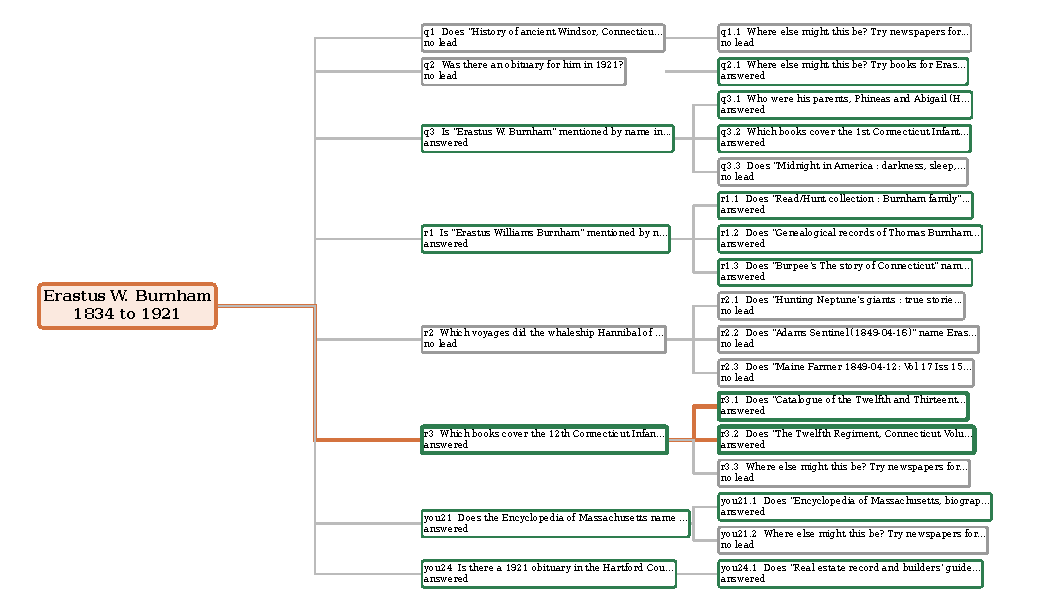
\includegraphics[width=0.92\textwidth,height=0.34\textheight,keepaspectratio]{figures/fig4-graph.pdf}
\caption{A real question graph (Erastus W.\ Burnham, 25 nodes), left to right: the person, then each question with its status written on the node. Highlighted: the 12th Connecticut chain, \textit{r3} (which books cover the regiment?) to \textit{r3.2} (does this book name him, on which page?), which reached the roster on page image 14. Ids \textit{r1} to \textit{r3} were re-asked from memory; \textit{you21} and \textit{you24} were injected by the reviewer.}
\label{fig:graph}
\end{figure*}

\subsection{Relation to prior search methods, and cost}
Tree of Thoughts searches over internal reasoning states with a model evaluator \citep{yao2023tot}; ReAct interleaves thought and action on one trajectory \citep{yao2023react}; Self-Ask decomposes a question into sub-questions \citep{press2023selfask}. CR differs in three ways: its nodes are questions to the outside world whose answers are evidence; generation is grounded in a cited finding; and the question set is persisted and reused across runs and subjects. Novelty search \citep{lehman2011novelty} and curiosity-driven exploration \citep{pathak2017curiosity,schmidhuber2010creativity} motivate rewarding novelty, but CR applies it to a question space with an external, verifiable payoff.

The graph has at most $\min(N,\sum_{k=1}^{d_{\max}} b^k)$ live nodes, plus up to 2 stub children per expanded node. Cost is linear in $|V|$ tool calls plus one generator call per expanded node. Event history also grows linearly in $|V|$: the 25-node run above ended at 303 events and 1.74\,MB of history. Week-long or 500-node runs need Temporal's continue-as-new with $(V,M)$ as compact state, or one child workflow per first-level subtree; neither is implemented yet.
